\documentclass[10pt,fleqn]{article}
\usepackage{hyperref}
\usepackage{graphicx}


\setlength{\topmargin}{-.75in}
\addtolength{\textheight}{2.00in}
\setlength{\oddsidemargin}{.00in}
\addtolength{\textwidth}{.75in}

\nofiles

\pagestyle{empty}

\setlength{\parindent}{0in}

% new math commands


\setlength{\oddsidemargin}{-0.25in}
\setlength{\evensidemargin}{-0.25in}
\setlength{\textwidth}{6.75in}
\setlength{\headheight}{0.0in}
\setlength{\topmargin}{-0.25in}
\setlength{\textheight}{9.00in}

\makeindex

\usepackage{mathrsfs}

%\usepackage[pdftex]{graphicx}
\usepackage{epstopdf}

\newcounter{beans}

\newcommand{\ds}{\displaystyle}
\newcommand{\limit}[2]{\displaystyle\lim_{#1\to#2}}

\newcommand{\binomial}[2]{\ \left( \begin{array}{c}
                                  #1 \\
                                  #2
                                 \end{array}
                            \right) \
                         }
\newcommand{\ExampleRule}[2]
  {
  \noindent
  \rule{\linewidth}{1pt}
  \begin{example}
    #1
    \label{#2}
  \end{example}
  \rule{\linewidth}{1pt}
  \vskip0.125in
  }

\newcommand{\defbox}[1]
  {
   \ \\
   \noindent
   \setlength\fboxrule{1pt}
   \fbox{
        \begin{minipage}{6.5in}
          #1
        \end{minipage}
        }
   \ \\
  }
\newcommand{\verysmallworkbox}[1]
  {
   \ \\
   \noindent
   \setlength\fboxrule{1pt}
   \fbox{
        \begin{minipage}{6.5in}
           #1
           \ \\
           \vskip0.5in \ \\
           \ \\
        \end{minipage}
        }
   \ \\
  }
\newcommand{\smallworkbox}[1]
  {
   \ \\
   \noindent
   \setlength\fboxrule{1pt}
   \fbox{
        \begin{minipage}{6.5in}
           #1
           \ \\
           \vskip2.5in \ \\
           \ \\
        \end{minipage}
        }
   \ \\
  }
\newcommand{\halfworkbox}[1]
  {
   \ \\
   \noindent
   \setlength\fboxrule{1pt}
   \fbox{
        \begin{minipage}{6.5in}
           #1 \hfill
           \ \\
           \vskip3.25in \ \\
           \ \\
        \end{minipage}
        }
   \ \\
  }
\newcommand{\largeworkbox}[1]
  {
   \ \\
   \noindent
   \setlength\fboxrule{1pt}
   \fbox{
        \begin{minipage}{6.5in}
           #1
           \ \\
           \vskip7.5in \ \\
           \ \\
        \end{minipage}
        }
   \ \\
  }
\newcommand{\flexworkbox}[2]
  {
   \ \\
   \noindent
   \setlength\fboxrule{1pt}
   \fbox{
        \begin{minipage}{6.5in}
           #1
           \ \\

           \vskip#2 \ \\
           \ \\
        \end{minipage}
        }
   \ \\
  }


% symbols for sets of numbers

\newcommand{\natnumb}{$\cal N$}
\newcommand{\whonumb}{$\cal W$}
\newcommand{\intnumb}{$\cal Z$}
\newcommand{\ratnumb}{$\cal Q$}
\newcommand{\irrnumb}{$\cal I$}
\newcommand{\realnumb}{$\cal R$}
\newcommand{\cmplxnumb}{$\cal C$}

% misc. commands

\newcommand{\mma}{{\it Mathematica}}
\newcommand{\sech}{\mbox{ sech}}
 
\newtheorem{theorem}{Theorem}
\newtheorem{example}{Example}
\newtheorem{definition}{Definition}
\newtheorem{problem}{Problem}

\setcounter{secnumdepth}{2}
\setcounter{tocdepth}{4}


\begin{document}
%%%%%%%%%%%%%%%%%%%%%%%%%%%%%%%%%%%%%%%%%%%%%%%%%%%%%%%%%%%%%%%%%%%%%%%%%%%%%%%%
%%%%%%%%%%%%%%%%%%%%%%%%%%%%%%%%%%%%%%%%%%%%%%%%%%%%%%%%%%%%%%%%%%%%%%%%%%%%%%%%
\vskip0.1in\hrule\vskip0.1in \noindent
{\bf Math 4610 Fundamentals of Computational Mathematics  - Topic 11.}
\vskip0.1in\hrule\vskip0.1in \noindent
In the last topic, a means for producing graphs for a single function that has
been hardwired into the Python module. It would be a lot better to have a module
or modules that can handle a little more generality in the function being
graphed. For this example, we might want to be able to enter a string that can
be used in place of the hardwired function with a general expression. The work
from the previous topic can be modified a bit to create a more general plotting
tool. In this topic, we will produce a couple of Python modules that will plot
(1) data from an input file and (2) use an input expression to produce a plot.
%%%%%%%%%%%%%%%%%%%%%%%%%%%%%%%%%%%%%%%%%%%%%%%%%%%%%%%%%%%%%%%%%%%%%%%%%%%%%%%%
%%%%%%%%%%%%%%%%%%%%%%%%%%%%%%%%%%%%%%%%%%%%%%%%%%%%%%%%%%%%%%%%%%%%%%%%%%%%%%%%
\vskip0.1in\hrule\vskip0.1in\noindent
{\bf Plotting Data From An Existing File: } 
\vskip0.1in\hrule\vskip0.1in\noindent
In this example, we will open and read a file into arrays of the coordinates
that represent ordered pairs. There is an age-old problem in the process of
loading data from a file system into a format that is recognized by the coding
language you use. As a simple example, Windows machines end lines using a
carriage return and Linux operating systems end lines in data files using the
new line character. These characters are usually hidden from you, but they are
really there. If you edit a file created using something like Notepad and then
open the file in vim the carriage return characters show up. If you go the other
way the new line characters are ignored and the lines are put one after the
other without breaks. There are a couple of commands that will transform back
and forth in this case. For example
\begin{verbatim}

    koebbe% dos2unix filename

\end{verbatim}
will transform the file and change carriage returns into new line characters.
This aside does not help with plotting functions. However, it is another little
trick that is worth knowing.

So, let's consider an input file that looks like:
\begin{verbatim}

      1, 3
      2, 4
      3, 17
      4, 2
      5, -3
      6, 4
      7, 6
      8, -2
      9, 3
     10, 0

\end{verbatim}
Each line in the file represents an ordered pair. So, the third line in the file
represents the ordered pair \((3, 17)\). So, the trick is to read in the ordered
pairs and use them to generate a plot.

A Python code that will do just that is included here. Note that there are a few
inputs that are required.
\begin{verbatim}

      from matplotlib import pyplot as plt
      import numpy as np
      #
      # initialize two arrays to store the data in
      # ------------------------------------------
      #
      xpts=[]
      ypts=[]
      #
      # user inputs a string for the name of the file containing the data
      # -----------------------------------------------------------------
      #
      datafilename = input('Enter the name of a data file:\n')
      #
      # the code expects ordered pairs, one per line in the file with a comma
      # separator - this is a very simple format
      # ----------------------------------------
      #
      xpts, ypts = np.loadtxt(datafilename, delimiter=',', unpack=True)
      #
      # the next block will ask for an expression for the data generation
      # ------------------------------------------
      #
      # now that the data is set up, we can do the graphics in the lines below
      #
      # set the maximum and minimum values for the graphing below
      # ---------------------------------------------------------
      #
      xmin = np.min(xpts)
      xmax = np.max(xpts)
      #
      # set the limits on the plot on the horizontal axis
      # -------------------------------------------------
      #
      plt.xlim(xmin, xmax)
      #
      # plot the data using matplotlib.pyplot
      # -------------------------------------
      #
      plt.plot(xpts, ypts, label='plot from data')
      #
      # create labels for the two axes in the 2-d plot
      # ----------------------------------------------
      #
      hlabel = input('Enter the label for the horizontal axis:\n')
      plt.xlabel(hlabel)
      vlabel = input('Enter the label for the vertical axis:\n')
      plt.ylabel(vlabel)
      #
      # create a title for the plot
      # ---------------------------
      #
      ptitle = input('Enter the title for the plot:\n')
      plt.title(ptitle)
      #
      # create a legend for the plot, if needed
      # ---------------------------------------
      #
      plt.legend()
      #
      # show the plot of the data
      # -------------------------
      #
      plt.show()
      #

\end{verbatim}
Once the data file is identified, there are a couple of important lines that
transform the input into actual numerical values. The use of the numpy package
will cast the strings read from the file into numerical values. This is done
as the file is read, in the code line
\begin{verbatim}

      xpts, ypts = np.loadtxt(datafilename, delimiter=',', unpack=True)

\end{verbatim}
Note that the syntax in Python allows the multiple assignment of array values.
xpts and ypts are initalized as arrays that allow an arbitrary number of values
to be appended to each.

In looking at the code, 4 inputs are required in order to have the code run to
completion. The one necessary input is the file name. The other three can be
anything including a blank string. So, as shown in the following figure, a file
name is input that accesses the ordered pairs given above. The labels are not
actually necessary. However, having labels always helps with graphs of
functions.
\vfill
\begin{figure}[h]
\centering
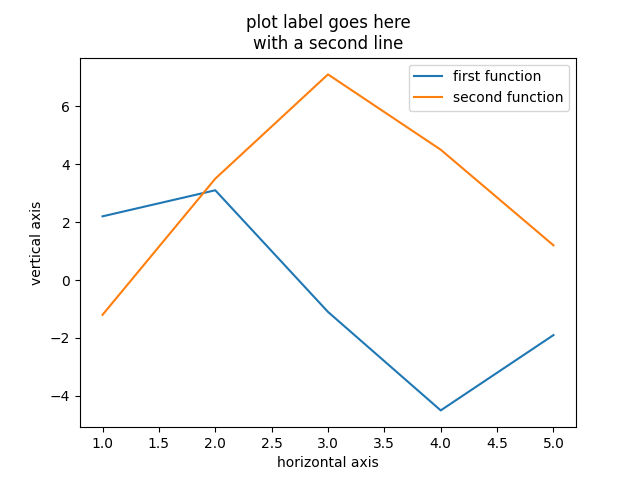
\includegraphics[width=6.0in]{../images/2ddataplot_01.png}
\vskip0.1in
\caption{A simple 2-d plot of data in an external file.
\end{figure}
\eject
The input needed to create the graph of the ordered pairs in the file are shown
in the following figure. Note that the 
\vfill
\begin{figure}[h]
\centering
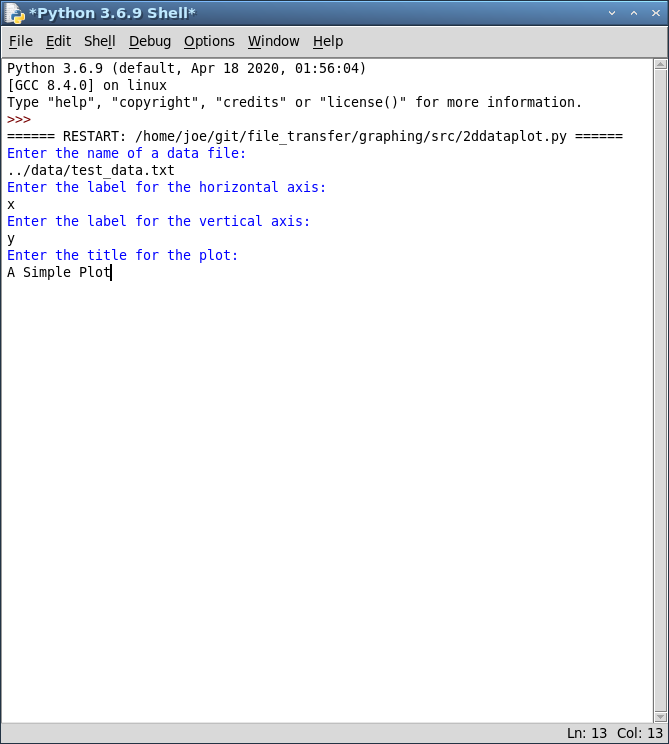
\includegraphics[width=6.0in]{../images/2ddataplot_02.png}
\vskip0.1in
\caption{The input needed to run the module and produce the plot of the data.}
\end{figure}
%%%%%%%%%%%%%%%%%%%%%%%%%%%%%%%%%%%%%%%%%%%%%%%%%%%%%%%%%%%%%%%%%%%%%%%%%%%%%%%%
%%%%%%%%%%%%%%%%%%%%%%%%%%%%%%%%%%%%%%%%%%%%%%%%%%%%%%%%%%%%%%%%%%%%%%%%%%%%%%%%
\vskip0.1in\hrule\vskip0.1in\noindent
{\bf Plotting Data from an Input String:} 
\vskip0.1in\hrule\vskip0.1in\noindent
\vfill
\begin{figure}[h]
\centering
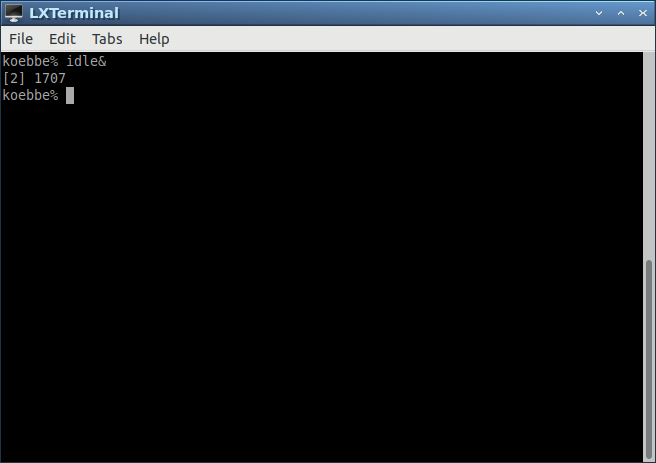
\includegraphics[width=6.0in]{../images/2dplot_02.png}
\vskip0.1in
\caption{Starting IDLE in a terminal emulator.}
\end{figure}
\eject
%%%%%%%%%%%%%%%%%%%%%%%%%%%%%%%%%%%%%%%%%%%%%%%%%%%%%%%%%%%%%%%%%%%%%%%%%%%%%%%%
%%%%%%%%%%%%%%%%%%%%%%%%%%%%%%%%%%%%%%%%%%%%%%%%%%%%%%%%%%%%%%%%%%%%%%%%%%%%%%%%
\vskip0.1in\hrule\vskip0.1in
\noindent
{\bf Opening a New File to Write Code} 
\vskip0.1in\hrule\vskip0.1in
\noindent
\vskip0.1in\hrule\vskip0.1in
\vfill
\begin{figure}[h]
\centering
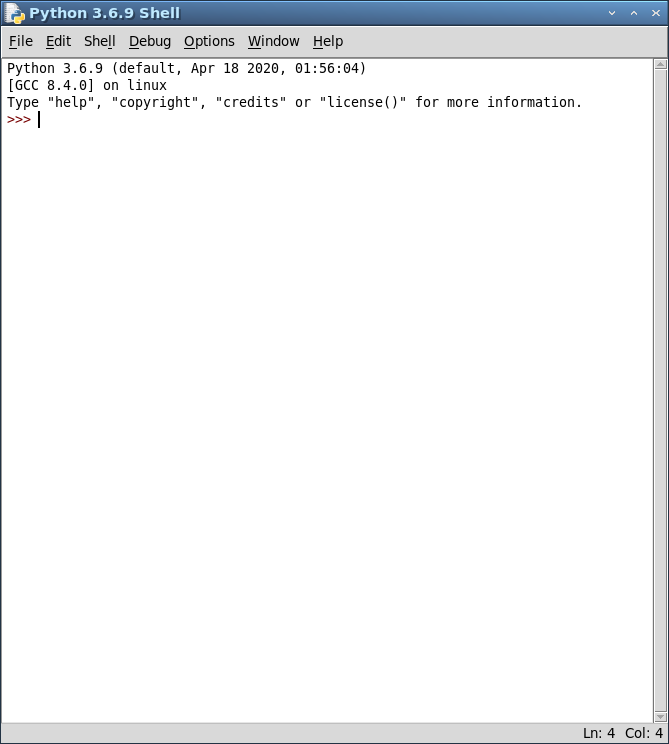
\includegraphics[width=6.0in]{../images/2dplot_03.png}
\caption{Opening a New File to write code in Python.}
\end{figure}
\eject
%%%%%%%%%%%%%%%%%%%%%%%%%%%%%%%%%%%%%%%%%%%%%%%%%%%%%%%%%%%%%%%%%%%%%%%%%%%%%%%%
%%%%%%%%%%%%%%%%%%%%%%%%%%%%%%%%%%%%%%%%%%%%%%%%%%%%%%%%%%%%%%%%%%%%%%%%%%%%%%%%
\vskip0.1in\hrule\vskip0.1in
\noindent
{\bf The Final Version of the Plotting Code in Python} 
\vskip0.1in\hrule\vskip0.1in\noindent
The next step is to type in Python code that will provide the 2-d plot that we
want.  The figure below shows the final code in the IDLE new file window. The
code can be run using the Run menu at the top of the window. When the module is
running you will be prompted to see if you want to save any changes to the code.
It is usually a good thing to save the changes.
\vskip0.1in\hrule\vskip0.1in\noindent

\begin{verbatim}

    #
    # import some stuff
    # -----------------
    #
    from matplotlib import pyplot as plt
    import numpy as np
    #
    # this is hardwired for a logistic function - so give initial time and final
    # time
    # ----
    #
    start = 0.0
    end = 20.0
    #
    # set an array of input/time values
    # ---------------------------------
    #
    t = []
    #
    # initialize a variable to keep track of the time at each iteration and append
    # the initial value to the array
    # ------------------------------
    #
    x = 0.0
    t.append(x)
    #
    # compute the time increment between samples
    # ------------------------------------------
    #
    dx = ( end - start ) / 201.
    #
    # set the functional form for the logistic solution
    # -------------------------------------------------
    #
    expression  = '(400.0 * np.exp(0.8*x)) / (500.0 + 3.0 * np.exp(0.8*x) )'
    #
    # initialize an array for the output/population density values
    # ------------------------------------------------------------
    #
    p = []
    p.append(eval(expression))
    #
    # set the loop iterator and start the while loop
    # ----------------------------------------------
    #
    l = 0
    while l < 200:
        #
        # compute the current value of the expression
        # -------------------------------------------
        #
        p.append(eval(expression))
        #
        # move on to the next value of the input
        # --------------------------------------
        #
        x = x + dx
        #
        # append the new value to the input array
        # ---------------------------------------
        #
        t.append(x)
        #
        # plus one the iterator
        # ---------------------
        #
        l += 1
    #
    # do the plot thing in matplotpy
    # ------------------------------
    #
    plt.xlabel('time values')
    plt.ylabel('population density values')
    plt.title('Logistic Population Growth Example')
    plt.plot(t, p)
    plt.show()

\end{verbatim}
\vskip0.1in\hrule\vskip0.1in\noindent
The code can be copied from these lecture notes and saved into a file. The
Python code is a hardwired version to graph the single expression
\begin{verbatim}

    expression  = '(400.0 * np.exp(0.8*x)) / (500.0 + 3.0 * np.exp(0.8*x) )'

\end{verbatim}
in python. It might be a good idea to write a general code. This will be done
in the next topic.
\vfill
\begin{figure}[h]
\centering
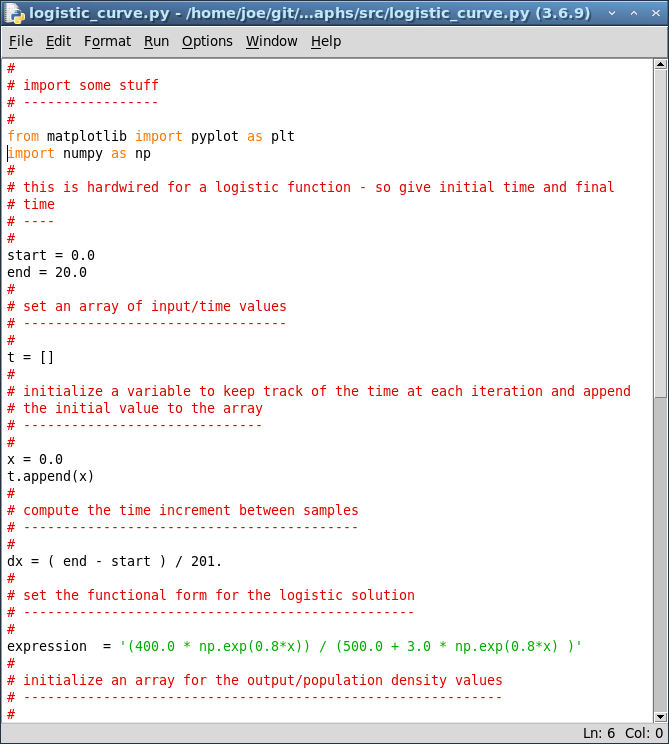
\includegraphics[width=6.0in]{../images/2dplot_05.png}
\caption{The final code in the window to produce a 2d-plot of a logistic
         population model.}
\end{figure}
\eject
%%%%%%%%%%%%%%%%%%%%%%%%%%%%%%%%%%%%%%%%%%%%%%%%%%%%%%%%%%%%%%%%%%%%%%%%%%%%%%%%
%%%%%%%%%%%%%%%%%%%%%%%%%%%%%%%%%%%%%%%%%%%%%%%%%%%%%%%%%%%%%%%%%%%%%%%%%%%%%%%%
\vskip0.1in\hrule\vskip0.1in\noindent
{\bf The Final Result} 
\vskip0.1in\hrule\vskip0.1in\noindent
When the Run menu item is selected, the result will be a new window popping up
that displays the graph in the first figure of this section of the notes.
The nice thing is that you can save a copy of the figure in several formats.
Your instructor usually likes a Portable Network Graphics (png) format. 
\vskip0.1in\hrule\vskip0.1in
\vfill
\begin{figure}[h]
\centering
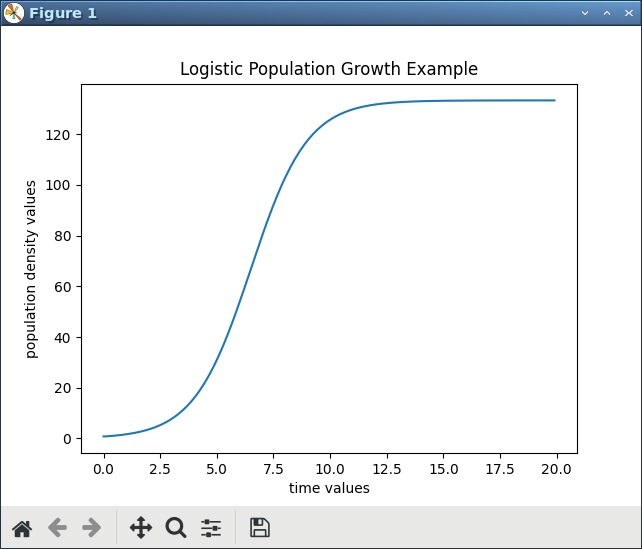
\includegraphics[width=6.0in]{../images/2dplot_06.png}
\caption{The output from the 2d plotting script is a window that shows the plot
         with a toolbar at the bottom of the window. The controls on the
         toolbar can be used to save a copy among other options.}
\end{figure}
\eject
%%%%%%%%%%%%%%%%%%%%%%%%%%%%%%%%%%%%%%%%%%%%%%%%%%%%%%%%%%%%%%%%%%%%%%%%%%%%%%%%
%%%%%%%%%%%%%%%%%%%%%%%%%%%%%%%%%%%%%%%%%%%%%%%%%%%%%%%%%%%%%%%%%%%%%%%%%%%%%%%%
\end{document} 
